\documentclass[10pt,aspectratio=169]{beamer}

\usetheme[progressbar=foot]{metropolis}
\AtBeginSection{}

\usepackage{appendixnumberbeamer}
\usepackage{booktabs}
\usepackage[scale=2]{ccicons}
\usepackage{tabularx}
\usepackage{tikz}
\usetikzlibrary{arrows.meta,positioning,shapes.geometric,fit}
\usepackage{xspace}
\newcommand{\themename}{\textbf{\textsc{metropolis}}\xspace}
\usepackage{comment}
\usepackage{caption}
\usepackage[
  backend=biber,
  style=authoryear
]{biblatex}

\setbeamertemplate{bibliography item}{}
\addbibresource{bibliography.bib}

\usepackage{graphicx}
\usepackage{siunitx}



%................................................................................
% COLORS

\definecolor{ukudlaBlue}{RGB}{41, 60, 135}
\definecolor{ukudlaLightBlue}{RGB}{212, 216, 231}
\definecolor{ukudlaRed}{RGB}{164, 28, 34}
\definecolor{ukudlaLightRed}{RGB}{236, 209, 210}
\definecolor{ukudlaGreen}{RGB}{59, 139, 71}
\definecolor{ukudlaLightGreen}{RGB}{215, 231, 218}
\definecolor{ukudlaYellow}{RGB}{239, 198, 44}
\definecolor{ukudlaLightYellow}{RGB}{251, 243, 212}
\definecolor{white}{RGB}{255, 255, 255}
\definecolor{black}{RGB}{0, 0, 0}

\setbeamercolor{palette primary}{fg=white, bg=ukudlaGreen}
\setbeamercolor{progress bar}{fg=ukudlaRed, bg=ukudlaYellow}
\setbeamercolor{title separator}{fg=ukudlaRed, bg=ukudlaYellow}
\setbeamercolor{progress bar in head/foot}{fg=ukudlaRed, bg=ukudlaYellow}
\setbeamercolor{progress bar in section page}{fg=ukudlaRed, bg=ukudlaYellow}
\setbeamercolor{background canvas}{bg=white}
\setbeamercolor{block body}{bg=ukudlaLightGreen,fg=black}



%................................................................................
% PRESENTATION INFORMATION

\title{UKUDLA Data Science Certificate}
\subtitle{Data Management}
\author{Markus Mößler}
\institute{University of Hohenheim}



%................................................................................
% CUSTOM FOOTER

\makeatletter
\setbeamertemplate{progress bar in head/foot}{%
  \tikzset{metropolis@progressbar@foreground/.style={fill=ukudlaGreen}}%
  \tikzset{metropolis@progressbar@background/.style={fill=ukudlaLightGreen}}%

  \begin{tikzpicture}[overlay, x=\paperwidth, y=1cm]
    \fill[metropolis@progressbar@background]
      (0,0) rectangle (1,0.10);
    \fill[metropolis@progressbar@foreground]
      (0,0) rectangle
      ({\insertframenumber/\inserttotalframenumber},0.10);
    \node[anchor=south west, yshift=0.25cm, xshift=0.2cm]
      at (0,0)
      {\includegraphics[height=0.75cm]{./logos/UKUDLA_logo_03_white_bg.pdf}};
    % current section
    \ifnum\value{section}>0
      \node[
        anchor=south east,
        yshift=0.22cm,
        xshift=-0.60cm,
        fill=ukudlaLightGreen,
        rounded corners=2pt,
        inner xsep=6pt,
        inner ysep=3pt,
        font=\scriptsize\bfseries,
        text=ukudlaRed
      ] at (1,0) {
        \insertsectionhead
      };
    \fi

  \end{tikzpicture}%
}
\makeatother



%................................................................................
% CUSTOM TITLE PAGE

\makeatletter
\setbeamertemplate{title page}{
  \begin{beamercolorbox}[sep=8pt, center, wd=\paperwidth, ht=0.5\paperheight]{title page top}
    \begin{minipage}[c]{1.00\textwidth}
      \raggedleft
      \includegraphics[height=1.00cm]{./logos/ukudla_universities.pdf}
      \vspace*{0.2cm}
    \end{minipage}
    \begin{beamercolorbox}[wd=0.9\paperwidth, sep=12pt, left]{top box}
      {\usebeamerfont{title}\usebeamercolor[fg]{title}\inserttitle\par}
      \vskip0.1cm
      {\usebeamerfont{subtitle}\usebeamercolor[fg]{subtitle}\insertsubtitle\par}
    \end{beamercolorbox}
  \end{beamercolorbox}
  \begin{beamercolorbox}[sep=8pt, center, wd=\paperwidth, ht=0.5\paperheight]{title page bottom}
    \begin{beamercolorbox}[wd=0.9\paperwidth, sep=12pt, left]{bottom box}
      \hbox{%
        \hspace*{1em}
        \begin{minipage}[c]{0.40\textwidth}
          \vskip1.0cm
          {\usebeamerfont{author}\usebeamercolor[fg]{author}\insertauthor\par}
          \vskip0.1cm
          {\usebeamerfont{institute}\usebeamercolor[fg]{institute}\insertinstitute\par}
        \end{minipage}%
        \hspace*{1.5cm}
        \begin{minipage}[c]{1.00\textwidth}
          \includegraphics[height=2.0cm]{./logos/UKUDLA_logo_05.pdf}
        \end{minipage}%
      }
    \end{beamercolorbox}
    \begin{minipage}[r]{1.00\textwidth}
      \centering
      \includegraphics[width=1.00\textwidth]{./logos/ukudla_sponsors.pdf}
    \end{minipage}
  \end{beamercolorbox}
}
\makeatother

\setbeamercolor{title page top}{bg=white}
\setbeamercolor{top box}{bg=ukudlaGreen}
\setbeamercolor{title page bottom}{bg=white}
\setbeamercolor{bottom box}{bg=ukudlaLightGreen}
\setbeamercolor{title}{fg=white}
\setbeamercolor{subtitle}{fg=white}
\setbeamercolor{author}{fg=black}
\setbeamercolor{institute}{fg=black}
\setbeamercolor{date}{fg=black}



%................................................................................
% DOCUMENT

\begin{document}

\maketitle

%--------------------------------------------------
{
\setbeamertemplate{frame numbering}[none]

\begin{frame}[noframenumbering]{Table of contents}

  \small
  \setbeamertemplate{section in toc}[sections numbered]
  \tableofcontents[hideallsubsections]

\end{frame}
}
%--------------------------------------------------



\section{Motivation}


%--------------------------------------------------
% CONTENT SLIDE 1/10
\begin{frame}{Reproducible analysis can reproduce a mistake}

\small

\begin{columns}[T]

\column{0.47\textwidth}

\textbf{The workflow runs}

\begin{itemize}
  \item code is versioned;
  \item packages are restored;
  \item the container starts; and
  \item the report is rendered.
\end{itemize}

\column{0.48\textwidth}

\textbf{But the data may be misunderstood}

\begin{itemize}
  \item a measurement uses the wrong unit;
  \item missing values are read as zero;
  \item flags are ignored; or
  \item a revised source replaces an earlier file.
\end{itemize}

\end{columns}

\vspace{0.35cm}

\begin{beamercolorbox}[rounded=true,sep=8pt]{block body}
Data management makes the meaning, origin, quality, organization, and permitted use of data explicit.
\end{beamercolorbox}

\end{frame}
%--------------------------------------------------


%--------------------------------------------------
% CONTENT SLIDE 2/10
\begin{frame}{Data move through a lifecycle}

\small
\centering

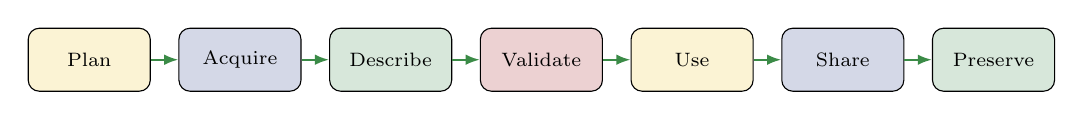
\begin{tikzpicture}[
  workflowstep/.style={
    draw,
    rounded corners,
    minimum width=1.55cm,
    minimum height=0.80cm,
    align=center,
    font=\scriptsize
  },
  arrow/.style={-{Latex[length=1.8mm]},thick,ukudlaGreen}
]
  \node[workflowstep,fill=ukudlaLightYellow] (plan) {Plan};
  \node[workflowstep,fill=ukudlaLightBlue,right=0.35cm of plan] (acquire) {Acquire};
  \node[workflowstep,fill=ukudlaLightGreen,right=0.35cm of acquire] (describe) {Describe};
  \node[workflowstep,fill=ukudlaLightRed,right=0.35cm of describe] (validate) {Validate};
  \node[workflowstep,fill=ukudlaLightYellow,right=0.35cm of validate] (use) {Use};
  \node[workflowstep,fill=ukudlaLightBlue,right=0.35cm of use] (share) {Share};
  \node[workflowstep,fill=ukudlaLightGreen,right=0.35cm of share] (preserve) {Preserve};
  \draw[arrow] (plan) -- (acquire);
  \draw[arrow] (acquire) -- (describe);
  \draw[arrow] (describe) -- (validate);
  \draw[arrow] (validate) -- (use);
  \draw[arrow] (use) -- (share);
  \draw[arrow] (share) -- (preserve);
\end{tikzpicture}

\vspace{0.55cm}

\raggedright

\begin{itemize}
  \item Decisions at one stage affect what is possible at later stages.
  \item Documentation and provenance connect the stages.
  \item Validation is repeated when data, requirements, or uses change.
\end{itemize}

\vspace{0.15cm}

\begin{beamercolorbox}[rounded=true,sep=8pt]{block body}
This session moves from \textbf{motivation}, through the essential
\textbf{concepts}, to their responsible \textbf{application} in a data workflow.
\end{beamercolorbox}

\end{frame}
%--------------------------------------------------



\section{Concepts}


%--------------------------------------------------
% CONTENT SLIDE 3/10
\begin{frame}{What does one row represent?}

\small

\begin{columns}[T]

\column{0.43\textwidth}

\textbf{Dataset grain}

The grain states what a single observation represents.

\vspace{0.20cm}

Depending on the study, one row may represent one:

\begin{itemize}
  \item sample or specimen;
  \item plot or observational unit;
  \item measurement occasion;
  \item experimental treatment; or
  \item reported entity and period.
\end{itemize}

\column{0.53\textwidth}

\begin{tabularx}{\textwidth}{lX}
\toprule
\textbf{Role} & \textbf{Example} \\
\midrule
Identifier & Sample, plot, farm or region ID \\
Time & Collection date, season or year \\
Measure & Observed value \\
Meaning & Variable or assay \\
Context & Unit, treatment, method or flag \\
\bottomrule
\end{tabularx}

\vspace{0.35cm}

\begin{beamercolorbox}[rounded=true,sep=7pt]{block body}
A key is the smallest set of variables expected to identify one row uniquely.
\end{beamercolorbox}

\end{columns}

\end{frame}
%--------------------------------------------------


%--------------------------------------------------
% CONTENT SLIDE 4/10
\begin{frame}{Food-systems evidence has different structures}

\small

\begin{columns}[T]

\column{0.48\textwidth}

\textbf{Study structures}

\begin{itemize}
  \item Laboratory: aliquots within samples or batches
  \item Experiment: treatments assigned to field units
  \item Observation: farms, plots or people measured without assignment
  \item Secondary: reported entities and periods
\end{itemize}

\column{0.48\textwidth}

\textbf{Common dimensions}

\begin{itemize}
  \item Cross-sectional, longitudinal or repeated measures
  \item Hierarchical units, blocks, sites and batches
  \item Points, polygons, transects or raster cells
  \item Identifiers, protocols and boundaries may change
\end{itemize}

\end{columns}

\vspace{0.35cm}

\begin{beamercolorbox}[rounded=true,sep=8pt]{block body}
Structure determines valid keys, comparisons, summaries, and integration choices. A file format alone does not describe that structure.
\end{beamercolorbox}

\end{frame}
%--------------------------------------------------



%--------------------------------------------------
% CONTENT SLIDE 5/10
\begin{frame}{Metadata and provenance answer different questions}

\small

\begin{columns}[T]

\column{0.31\textwidth}

\textbf{Source metadata}

\begin{itemize}
  \item definitions;
  \item methods;
  \item classifications;
  \item code lists; and
  \item quality flags.
\end{itemize}

\column{0.31\textwidth}

\textbf{Data dictionary}

\begin{itemize}
  \item variable names;
  \item meanings;
  \item types;
  \item units; and
  \item allowed values.
\end{itemize}

\column{0.33\textwidth}

\textbf{Provenance record}

\begin{itemize}
  \item collector or provider and dataset;
  \item protocol/version and collection/access date;
  \item license;
  \item retrieval method; and
  \item derived artifacts.
\end{itemize}

\end{columns}

\vspace{0.35cm}

\centering
\textcolor{ukudlaRed}{Metadata explain data; provenance explains their history.}

\end{frame}
%--------------------------------------------------


%--------------------------------------------------
% CONTENT SLIDE 6/10
\begin{frame}{Data quality means fitness for purpose}

\small

\centering

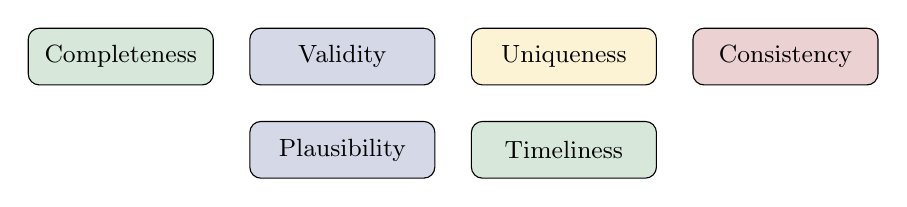
\begin{tikzpicture}[
  quality/.style={
    draw,
    rounded corners,
    minimum width=2.35cm,
    minimum height=0.72cm,
    align=center,
    font=\small
  }
]
  \node[quality,fill=ukudlaLightGreen] (complete) {Completeness};
  \node[quality,fill=ukudlaLightBlue,right=0.45cm of complete] (valid) {Validity};
  \node[quality,fill=ukudlaLightYellow,right=0.45cm of valid] (unique) {Uniqueness};
  \node[quality,fill=ukudlaLightRed,right=0.45cm of unique] (consistent) {Consistency};
  \node[quality,fill=ukudlaLightBlue,below=0.45cm of valid] (plausible) {Plausibility};
  \node[quality,fill=ukudlaLightGreen,right=0.45cm of plausible] (timely) {Timeliness};
\end{tikzpicture}

\vspace{0.45cm}

\raggedright

\begin{itemize}
  \item Quality requirements depend on the research question and intended use.
  \item Accuracy often cannot be established from a file alone.
  \item Field notes, laboratory flags and provider notes are part of the evidence.
  \item A quality concern should be reported before it is corrected or excluded.
\end{itemize}

\end{frame}
%--------------------------------------------------


\section{Application}


%--------------------------------------------------
% CONTENT SLIDE 7/10
\begin{frame}{Application: validate before transforming}

\small

\begin{columns}[T]

\column{0.47\textwidth}

\textbf{Structural checks}

\begin{itemize}
  \item expected columns and types;
  \item row count and temporal coverage;
  \item uniqueness of the proposed key;
  \item duplicate records; and
  \item allowed codes and units.
\end{itemize}

\column{0.47\textwidth}

\textbf{Semantic checks}

\begin{itemize}
  \item missingness patterns;
  \item impossible or suspicious values;
  \item consistency with definitions;
  \item agreement with metadata; and
  \item unresolved quality flags.
\end{itemize}

\end{columns}

\vspace{0.35cm}

\begin{beamercolorbox}[rounded=true,sep=8pt]{block body}
Validation should reveal assumptions and anomalies. It should not silently ``fix'' the evidence.
\end{beamercolorbox}

\end{frame}
%--------------------------------------------------



%--------------------------------------------------
% CONTENT SLIDE 8/10
\begin{frame}[fragile]{Organize the project by data role}

\scriptsize

\begin{columns}[T]

\column{0.43\textwidth}

\begin{verbatim}
analysis-project/
|-- data-raw/
|-- data-interim/
|-- data-processed/
|-- metadata/
|-- scripts/
`-- reports/
\end{verbatim}

\column{0.53\textwidth}

\small

\begin{itemize}
  \item Preserve raw inputs unchanged.
  \item Create derived data with code.
  \item Keep dictionaries, licenses and provenance near the project.
  \item Use stable names, not \texttt{final-v2-revised.csv}.
  \item Decide deliberately which data belong in Git.
\end{itemize}

\end{columns}

\vspace{0.30cm}

\begin{beamercolorbox}[rounded=true,sep=8pt]{block body}
Raw, interim and processed describe roles in a workflow---not levels of correctness.
\end{beamercolorbox}

\end{frame}
%--------------------------------------------------


%--------------------------------------------------
% CONTENT SLIDE 9/10
\begin{frame}{Manage the project data responsibly}

\small

\begin{columns}[T]

\column{0.47\textwidth}

\textbf{Before storing or sharing}

\begin{itemize}
  \item Check consent, license and terms of use.
  \item Record citation and attribution.
  \item Confirm whether redistribution is permitted.
  \item Protect personal, confidential and location-sensitive data.
\end{itemize}

\column{0.47\textwidth}

\textbf{FAIR principles}

\begin{itemize}
  \item Findable
  \item Accessible
  \item Interoperable
  \item Reusable
\end{itemize}

\vspace{0.15cm}

FAIR does not necessarily mean open.

\end{columns}

\vspace{0.25cm}

\begin{beamercolorbox}[rounded=true,sep=8pt]{block body}
Farm, household, location and biological data can remain sensitive even after direct names are removed.
\end{beamercolorbox}

\end{frame}
%--------------------------------------------------



%--------------------------------------------------
\section{Key Message}
% CONTENT SLIDE 10/10

\begin{frame}{Key message: make data inspectable before analysis}

\small

\centering

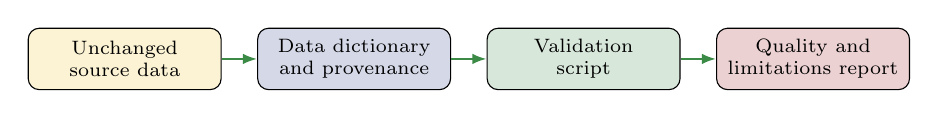
\begin{tikzpicture}[
  artifact/.style={
    draw,
    rounded corners,
    minimum width=2.45cm,
    minimum height=0.78cm,
    align=center,
    font=\scriptsize
  },
  arrow/.style={-{Latex[length=1.8mm]},thick,ukudlaGreen}
]
  \node[artifact,fill=ukudlaLightYellow] (raw) {Unchanged\\source data};
  \node[artifact,fill=ukudlaLightBlue,right=0.45cm of raw] (dictionary) {Data dictionary\\and provenance};
  \node[artifact,fill=ukudlaLightGreen,right=0.45cm of dictionary] (checks) {Validation\\script};
  \node[artifact,fill=ukudlaLightRed,right=0.45cm of checks] (report) {Quality and\\limitations report};
  \draw[arrow] (raw) -- (dictionary);
  \draw[arrow] (dictionary) -- (checks);
  \draw[arrow] (checks) -- (report);
\end{tikzpicture}

\vspace{0.45cm}

\raggedright

\begin{enumerate}
  \item State the grain and expected key.
  \item Interpret variables, units, codes and flags.
  \item Document source, meaning, license and history.
  \item Validate structure and meaning without changing the raw file.
  \item Record unresolved concerns for the next workflow stage.
\end{enumerate}

\vspace{0.15cm}

\centering
\textcolor{ukudlaRed}{The next session asks how to obtain and integrate multiple sources.}

\end{frame}
%--------------------------------------------------


%--------------------------------------------------
\begin{frame}[plain,noframenumbering]{Supported by}

  South African government and the National Research Foundation

  \begin{flushleft}
    \includegraphics[trim=0cm 0cm 0cm 0cm, clip, width=0.50\textwidth]{./logos/ukudla_south_african_sponsors.pdf}
  \end{flushleft}

  German government and the German Academic Exchange Service

  \begin{flushleft}
    \includegraphics[trim=0cm 0cm 0cm 0cm, clip, width=1.00\textwidth]{./logos/ukudla_german_sponsors.pdf}
  \end{flushleft}

\end{frame}
%--------------------------------------------------

\end{document}
